\chapter{Machine Learning on RE}
\label{chap:ml}
RE are big part of language realization of a navigation system and especially so in the GIVE scenario. My work attempts to apply machine learning techniques on S-GIVE dataset with a clear goal to help navigation system with RE. These attempts are presented in this chapter.

Machine learning (ML) is becoming a popular topic together with a very broad term of Big Data. This branch of artificial intelligence encompasses various problems such as classification or clustering. Research in the area of ML spawned various algorithms for solving these problems and evaluation techniques for comparing the models outputted by the learning process. 

It is important to emphasize that ML creates models which can only be as good as the data they were trained on. Careful and thorough data analysis is crucial part of ML process. When it comes to feature extraction, experimentation are sometimes the only method for finding better models. 

In the first section I'll describe attempts at predicting timing of the first reference to a target button. 

Second section talks about modeling of chains of references. 
Third section briefly touches a topic of using room memory. 

In the last section, I will present my thoughts on the results of previous sections.

\section{Timing of the first reference}
\label{sec:timing-firsref-ml}
Work of \citet{stoia2006sentence} was previously mentioned in related work section of chapter \ref{chap:bg}. They applied machine learning on timing of the first reference in a 3D virtual world. The set-up of their experiment is quite similar to the GIVE's one and so I decided it would be interesting to replicate their methodology on GIVE dataset. 

I defined the problem of the timing of the first reference as a classification task, as did \citet{stoia2006sentence}. More precisely binary classification, the two classes being either refer to the target button or delay the reference. After extracting the first references to buttons which needed to be pressed from the dataset, I excluded plural references, because of their complexity. Some buttons were placed on top of each other and IG wasn't sure which one need to be pressed. These were excluded as well because of the unnecessary confusion. That left me with 351 first references. For each first reference I have chosen one negative example, where IG could refer to the target but chose not to. I picked negative examples randomly from interval between entering room and time of the first reference. Overall, that is 702 data-points with perfectly balanced classes.

As for features extraction, I have chosen similarly to \citet{stoia2006sentence} various spatial information. For the positive examples, I averaged these spatial information over 0.6 seconds window centered on the time of the reference. Reasoning for that, is that IG take scene situation into consideration before and possibly after they start uttering the reference. For negative examples I chose not to averaged them, since they are chosen randomly. All features are listed in the following list. The list also includes figures' numbers. These figures are histograms of the attributes, separated for both classes and can be found in appendix.

\begin{itemize}
\item
Distance to target button - Figure \ref{fig:fref-distrib-dist}
\item
Absolute value of angle to target - Figure \ref{fig:fref-distrib-angle}
\item
Whether target is visible (True/False) - Figure \ref{fig:fref-distrib-visib}
\item
Number of distractors - Figure \ref{fig:fref-distrib-distractors}
\item
Number of distracting buttons - Figure \ref{fig:fref-distrib-distbuttons}
\item
Number of visible buttons with smaller angle to IF than the target button - Figure \ref{fig:fref-distrib-distangles}
\end{itemize}

Once I have extracted these features I used three machine learning techniques: C4.5 decision tree because of their easy interpretation, naive Bayes to observe effect of all attributes and Support vector machine for linear classification. I used Weka software implementation of previous algorithms \citep{hall2009weka}.

For all the algorithms I used a standard ten-fold cross validation. The results can be seen in table \ref{tab:firstref}. Pruned decision tree for timing of the first reference can be seen in Figure \ref{fig:dectree}. I used two simple baselines to compare the results with. I have perfectly balanced classes so the first baseline is 50\%. Simple rule for the first reference is to refer when the target is visible, and delay it if the target is not visible. In my case that rule has an accuracy of 64.2\%. 

\begin{table}[!htbp]
 \centering
\begin{tabular}{lr}
\toprule
Model    & Accuracy (\%)  \\
\midrule
Class baseline    & 50.00\\
Visibility baseline & 64.2\\
\midrule
Naive Bayes  & \textbf{64.70} \\
C4.5 & 63.31 \\
SVM & 55.42 \\
\bottomrule
\end{tabular}
\caption{Results of first reference timing modeling}
\label{tab:firstref}
\end{table}

Only one algorithm was able to get over visibility baseline and not by a significant amount. These results were surprising, because \citet{stoia2006sentence} had success with the same approach on a similar dataset. Reasons for this difference are probably in the differences between their experiment and GIVE set-up. First, their tasks also included different actions than pushing buttons (e.g. picking up items). Second, their worlds had higher diversity of the distractors and smaller frequency of them. With increasing number of distractors and particularly distractors of the same category, it seems that spatial features loose their power in predicting the timing of the first reference. The number of visible distractors was the best attribute in their decision tree, but in my tree (figure \ref{fig:dectree}) it had lower information gain. Moreover, the decision tree did the split on the number of visible buttons not the number of all visible distractors.

After the timing of the first references classification proved to be more difficult than excepted, I have switched from predicting the timing of the references to predicting their content. Next, I focused on chains of references.

\begin{figure}[!htbp]
 \centering
\small
\begin{verbatim}
Distance to target <= 4.45
| Is target visible? = False: DELAY
| Is target visible? = True
| | Distance to target <= 2.51: REFER
| | Distance to target > 2.51
| | | Number of distracting buttons <= 4.67: REFER
| | | Number of distracting buttons > 4.67: DELAY
Distance to target > 4.45: DELAY
\end{verbatim}
\caption{Decision tree for first reference timing}
\label{fig:dectree}
\end{figure}

\section{Chains of references}
Section \ref{sec:dataset-chains} introduced the phenomenon of chains of references. It also analysed various linguistic functions the chains can play in REG. This section will build on top of this analysis, by employing machine learning techniques to model the chains.

Valid and important question is whether chains aren't something, which should actually be avoided, instead of modelled. That is, what is the relation between usage of chains and task performance measure, such as duration. To address this issues, I used linear regression predicting the duration of the experiment explained by the average chain length. Figure \ref{fig:chains_dur_scatter} does contain a hint of a trend, but also contains a lot of counter-examples. 

\begin{figure}[!htbp]
  \centering
	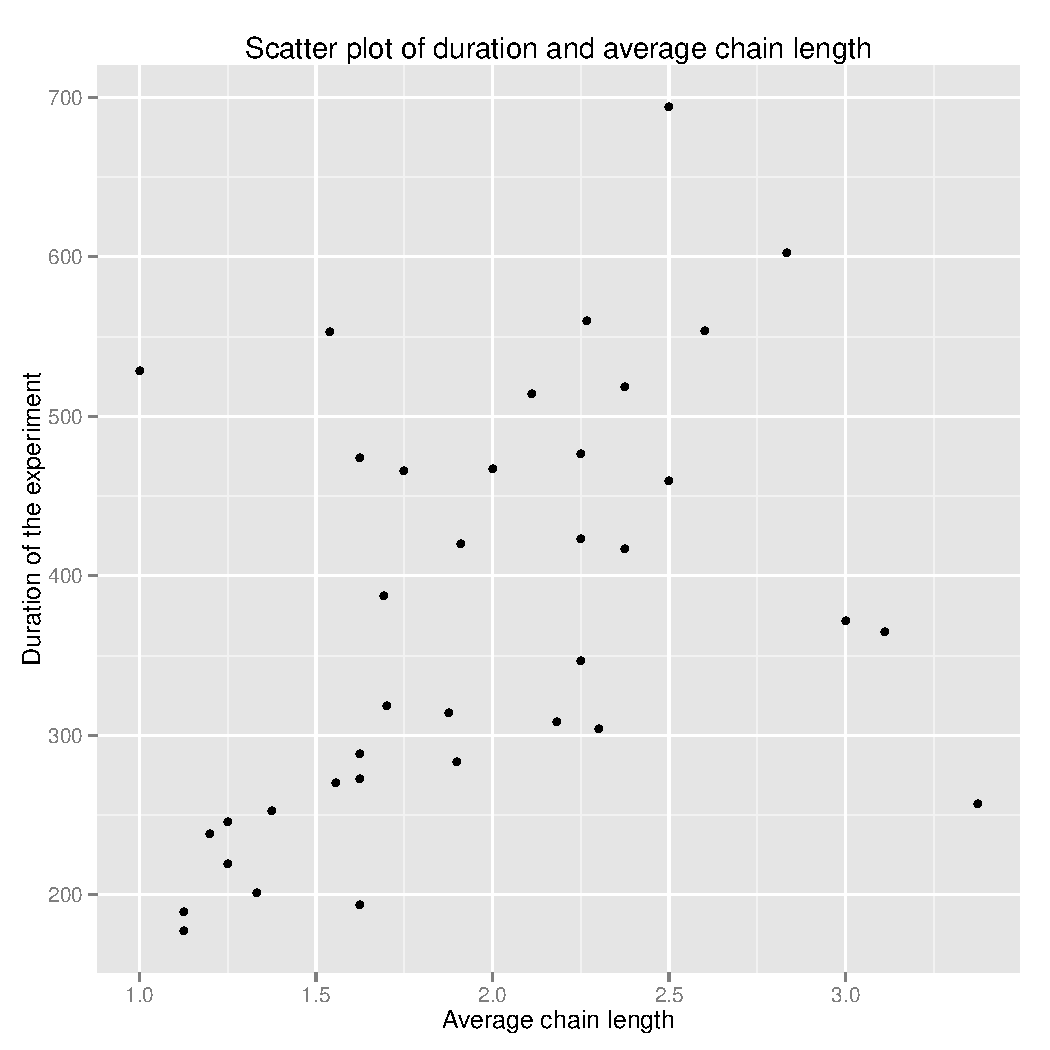
\includegraphics[width=0.8\textwidth]{Images/chains_duration_LR}
	\caption{Scatter plot of duration and chain length}
	\label{fig:chains_dur_scatter}
\end{figure}

When I applied linear regression the $R^2$ was 0.188, which means the average chain length explains very little of the duration variation. If the average chain length was to significantly influence the duration, I would except much higher $R^2$. Correlation between the duration and average chain length is not low: 0.433, however correlation does not imply causation. Longer chains can be caused by errors of IF or IG and the errors are also likely to increase the duration. Based on these facts, I don't believe the chains are harmful phenomenon and it makes sense to proceed with attempting to model them. 

With modeling the chains of references, there are numerous problems to tackle. Simple presence of the chain can be thought of as a classification task. It can be interesting try to predict the chain length. Having established common linguistic functions of the chains, classify chains whether they would contain these function is another task to consider. I looked into each of these problem. Trough extracting relevant features I thoroughly explored using machine learning for modeling the chains.

As a side note, during exploring chains of references I switched from Weka implementation of machine learning techniques \citep{hall2009weka} to scikit learn package for Python \citep{scikit-learn}. The main reason being easier automation of the entire pipeline, therefore speeding-up of the whole process and also more control over whole process.

\subsection{Presence of the chains}
From Section \ref{sec:dataset-chains}, the functions the chains can play in a discourse are known. However, what role does play the scene complexity and particular game state in the presence of the chains? Will more complex scene spawn more chains or are the chains too complex to be captured by simply looking at where they are created? To answer these question, I extracted scene complexity features and the target button for all references and classified whether the chains was present or not.

The features I extracted from the dataset are in the following list:

\begin{itemize}
\item
Target button	
\item
Number of objects In the room - Figure \label{fig:chains-distrib-objects}
\item
Number of buttons in the room - Figure \label{fig:chains-distrib-buttons}
\item
Number of landmarks in the room - Figure \label{fig:chains-distrib-landmarks}
\item
Number of very close buttons to the target button (closer than 0.3m) - Figure \label{fig:chains-distrib-veryclose}
\item
Number of buttons on the same wall as target button - Figure \label{fig:chains-distrib-samewall}
\item
Number of close buttons to the target button (closer than 1m) - Figure \label{fig:chains-distrib-close}
\item
Number of far buttons (farther than 1.5m) - Figure \label{fig:chains-distrib-far}
\end{itemize}

The target button is a categorical feature, so I used DictVectorizer class in scikit to transform it into multiple numerical features. I further tried to use all features, select 8 best features using SelectKBest class from scikit with $\chi^2$ statistic as a scoring function and select 16 best features using the same strategy. For algorithms I used Decision Tree, Naive Bayes, Support Vector Machines (SVM), One-Nearest Neighbour (1-NN), Two-Nearest Neighbours (2-NN) and Random Forest. This selection employs various approaches for classification task, each of the algorithms having strong and weak points. For evaluation, I used standard ten-fold cross validation and compared the accuracy of the classifiers with majority class baseline. From now on, I will also include double the standard deviation (std). The idea behind the double is that if the features follow normal distribution and the three sigma rule is applied, the chance of the accuracy being in interval of $\pm$ standard deviation times two is 95.45\% . The results are summarized in Table \ref{tab:chains-ml-presence}. 

\begin{table}[!htbp]
 \centering
\begin{tabular}{lccc}
\toprule
Features & Model    & Mean accuracy (\%) & $2\times$ std \\
\midrule
Majority baseline &    & 55.2	& \\
\midrule
All & Decision Tree 	& 55.5		& 13.5 	\\
	& Naive Bayes  	& 55.8		& 6.6 	\\
	& SVM 			& 56.1		& 11.2 	\\
	& 1-NN			& 56.3		& 9.3 	\\
	& 2-NN			& 53.6		& 12.1 	\\
	& Random Forest	& 55.0		& 13.6	\\
\midrule
8 best 	& Decision Tree 	& 	59.7		& 14.6  	\\
		& Naive Bayes  	&	56.4		& 2.9 	\\
		& SVM 			&	58.3		& 13.1 	\\
		& 1-NN			&	58.8		& 11.1 	\\
		& 2-NN			&	56.1		& 14.4 	\\
		& \textbf{Random Forest}	&	\textbf{60.0	}	& 16.6 	\\
\midrule
16 best & Decision Tree 	& 55.8	& 13.5  	\\
	& Naive Bayes  		& 56.4	& 2.9 	\\
	& SVM 				& 58.3	& 13.9  	\\
	& 1-NN				& 56.9	& 9.1  	\\
	& 2-NN				& 53.3	& 12.8  	\\
	& Random Forest		& 57.2	& 12.8  	\\	
\bottomrule
\end{tabular}
\caption{Results of chains presence modeling}
\label{tab:chains-ml-presence}
\end{table}

The best mean accuracy had the Random Forest for 8 best features. However, it wasn't significantly better than majority class baseline. Take into account the standard deviation, none of the classifier and features combination outperformed the baseline.  From these results, I conclude that the chains presence is not dependent only on the scene complexity and specific scenarios. IG strategies for referencing, IF behaviour and other circumstances play role in creation of the chains.

\subsection{Chain length prediction}
After not being able to predict presence of the chains based on spatial information and target button, I was interested if I could predict the chain length based. I used same attributes as in previous classification of the chains' presence, but added two more features concerned with IF movement behaviour. Namely, the ratio of the time IF spent not moving at all through the chain duration and ratio of the time IF spent only rotating in place through the chain duration. The idea behind these features is that IF who is not moving or just looking around is an indication of him/her being confused, which then should produce more referring expression for the chain.

For reference, I list all features and add figures numbers for the two new attributes:
\begin{itemize}
\item
Target button	
\item
Number of objects In the room
\item
Number of buttons in the room
\item
Number of landmarks in the room
\item
Number of very close buttons to the target button (closer than 0.3m)
\item
Number of buttons on the same wall as target button
\item
Number of close buttons to the target button (closer than 1m)
\item
Number of far buttons (farther than 1.5m)
\item
Ratio of time IF spent not moving - Figure \label{fig:chains-distrib-stop}
\item
Ratio of time IF spent rotating - Figure \label{fig:chains-distrib-rotate}
\end{itemize}

I applied linear regression, predicting chain length based on three groups of mentioned attributes - target, spatial features and IF movement behaviour features. I evaluated the regressions by looking at $R^2$. The results are in Table \ref{tab:chains-lr-length}.

\begin{table}[!htbp]
 \centering
\begin{tabular}{lc}
\toprule
Features & $R^2$  \\
\midrule
Target button & 0.154\\
Spatial & 0.146 \\
IF movement & 0.126 \\
Spatial ad IF movement & 0.262 \\
\bottomrule
\end{tabular}
\caption{Results of chains length modeling}
\label{tab:chains-lr-length}
\end{table}

None of the regressions from Table \ref{tab:chains-lr-length} are particularly good at predicting chain length. Combining spatial and IF movement features does increase the percentage of chain length variation explained by the model, suggesting that these features have, however small, effect on the chain length. Once again it shows that chains are complex phenomenon, influenced by IF, IG and scene variables.

\subsection{Closer look at chains' content}
Despite not being able to predict the chains presence and length, I was still interested in chains and decided to look closely into chains content. First, I took advantage of having annotated the functions in the chains, as introduced in Section \ref{sec:dataset-chains}. I focused on specification and group function and tried to predict whether the chain will contain these functions. Second, I tried to predict whether the chain provide new information about the target button after its first reference. For example IG could add RE about position of the target button relative to a landmark in the third reference of the chain. Reasoning behind this classification is trying to predict when IG add information to the chains.

For all these classification task, I used the same features as in the chain length prediction, that is: the target button, spatial features, IF movement behaviour features and combination of the previous two. Again, I used ten-fold cross validation for evaluation and compared that to majority class baseline. The results for specification function are in Table \ref{tab:chains-ml-specification}, for group function in Table \ref{tab:chains-ml-group} and for predicting new information in Table \ref{tab:chains-ml-infgain}. For algorithms, I maintained broad range of algorithms, similarly to previous machine learning attempts.

\begin{table}[!htbp]
 \centering
\begin{tabular}{lccc}
\toprule
Features & Model    & Mean accuracy (\%) & $2\times$ std (\%) \\
\midrule
 Majority baseline &   & 74.7	& \\
\midrule
Target button 	& Decision Tree 	& 73.3		& 6.0 	\\
				& Naive Bayes  	& 38.0		& 22.4	\\
				& SVM 			& 74.7		& 5.3 	\\
				& 1-NN			& 70.7		& 14.8 	\\
				& Random Forest	& 74.0		& 7.2	\\
\midrule
IF movement	& Decision Tree 	& 	64.0	& 21.7 \\
			& Naive Bayes  	&	72.7	& 11.1	\\
			& SVM 			&	74.7	& 5.3 	\\
			& \textbf{1-NN}			&	\textbf{77.3	} & 12.2 	\\
			& Random Forest	&	71.3	& 16.9 	\\
		
\midrule
Spatial	 	& Decision Tree 	& 74.7	& 16.7 \\
			& Naive Bayes  	& 66.7 	& 20.7	\\
			& SVM 			& 71.3	& 14.7 	\\
			& 1-NN			& 68.7	& 23.9 \\
			& Random Forest	& 74.7	& 18.7 \\	
\midrule
Spatial and movement& Decision Tree 	& 66.7	& 23.1 \\
					& Naive Bayes  	& 66.7	& 20.7	\\
					& SVM 			& 71.3	& 18.9 	\\
					& 1-NN			& 76.7	& 8.9 \\
					& Random Forest	& 68.0	& 16.7 \\			
\bottomrule
\end{tabular}
\caption{Results of specification function in chains modeling}
\label{tab:chains-ml-specification}
\end{table}

\begin{table}[!htbp]
 \centering
\begin{tabular}{lccc}
\toprule
Features & Model    & Mean accuracy (\%) & $2\times$ std (\%) \\
\midrule
Majority baseline &   & 75.4	& \\
\midrule
Target button 	& Decision Tree 	& 81.3		& 14.4 	\\
				& Naive Bayes  	& 38.0		& 14.7	\\
				& SVM 			& 75.3		& 6.1 	\\
				& 1-NN			& 79.3		& 13.9 	\\
				& Random Forest	& 79.3		& 17.3	\\
\midrule
IF movement	& Decision Tree 	& 	61.3	& 23.7 \\
			& Naive Bayes  	&	75.3	& 6.1	\\
			& SVM 			&	75.3	& 6.1 	\\
			& 1-NN			&	73.3	 & 15.8 	\\
			& Random Forest	&	68.0	& 16.7 	\\
\midrule
Spatial	 	& Decision Tree 	& 80.0	& 10.3 \\
			& Naive Bayes  	& 77.3 	& 18.1	\\
			& SVM 			& 77.3	& 8.8 	\\
			& 1-NN			& 77.3	& 13.6 \\
			& \textbf{Random Forest}	& \textbf{82.0}	& 13.4 \\	

\midrule
Spatial and movement& Decision Tree 	& 71.3	& 16.9 \\
					& Naive Bayes  	& 78.0	& 15.8	\\
					& SVM 			& 77.3	& 8.8 	\\
					& 1-NN			& 79.3	& 9.3 \\
					& Random Forest	& 74.0	& 18.3 \\	 	
\bottomrule
\end{tabular}
\caption{Results of group function in chains modeling}
\label{tab:chains-ml-group}
\end{table}

\begin{table}[!htbp]
 \centering
\begin{tabular}{lccc}
\toprule
Features & Model    & Mean accuracy (\%) &  $2\times$ std (\%) \\
\midrule
 Majority baseline  &   & 67.3	& \\
\midrule
Target button 	& Decision Tree 	& 68.3	& 19.6 	\\
				& Naive Bayes  	& 38.0	& 15.8	\\
				& SVM 			& 67.3	& 4.0 	\\
				& 1-NN			& 56.0	& 31.1 	\\
				& Random Forest	& 68.0	& 19.6	\\
\midrule
IF movement	& Decision Tree 	& 	58.7	& 8.0 \\
			& Naive Bayes  	&	68.0	& 11.6	\\
			& SVM 			&	67.3	& 4.0 	\\
			& 1-NN			&	41.3	& 20.5 	\\
			& Random Forest	&	57.3& 12.2 	\\
			
\midrule
Spatial	 	& Decision Tree 	& 68.0	& 16.7 \\
			& Naive Bayes  	& 60.7 	& 28.3	\\
			& SVM 			& 71.3	& 8.5 	\\
			& 1-NN			& 59.3	& 21.9 \\
			& Random Forest	& 67.3	& 17.3 \\	

\midrule
Spatial and movement& Decision Tree 	& 66.0	& 26.3 \\
					& Naive Bayes  	& 62.7	& 26.1	\\
					& \textbf{SVM} 	& \textbf{72.7}	& 9.3 	\\
					& 1-NN			& 59.3	& 19.3 \\
					& Random Forest	& 64.7	& 18.9 \\	 	
\bottomrule
\end{tabular}
\caption{Results of new information in chains modeling}
\label{tab:chains-ml-infgain}
\end{table}

The best classifiers for these 3 tasks can be found in respective results tables, marked by bold font. Similarly to previous attempts, all combinations of attributes and algorithms had the accuracy around the baseline. The last section of this chapter will address these and all previous results in more depth. But before that, I modeled one more subtask, which is introduced in following section

\section{Room memory}
\label{sec:room-memory-ml}
Last machine learning problem I tackled was using memory of the previously visited rooms in RE for room switching. When IF has to return to a recently visited room, IG sometimes employ RE such as: ``Go to the room you were just in.'' Deciding whether to use the memory in room switching RE can be thought of as a classification task.

I extracted all moments where IF went between rooms and determined whether the room memory was used from what was IG saying before going into the new room. I also extracted 3 features:

\begin{itemize}
\item
Was IF in the new room before?
\item
How many seconds before, he/she was there?
\item
How many rooms before, he/she was there?
\end{itemize}

The last feature being of a categorical character, once again DictVectorizer was used for transformation and from the transformed numerical values I selected 3 best with SelectKBest and $\chi^2$ statistic. The results are in Table \ref{tab:history-ml}.

\begin{table}[!htbp]
 \centering
\begin{tabular}{lcc}
\toprule
Model    & Mean accuracy (\%) & $2\times$ Std (\%) \\
\midrule
 Majority baseline    & 78.5	& \\
\midrule
 Decision Tree 	& 78.0	& 7.1 	\\
 Naive Bayes  	& 68.3	& 7.3	\\
 SVM 			& 82.2	& 6.2 	\\
 1-NN			& 80.8	& 6.6 	\\
 \textbf{Random Forest}	& \textbf{84.4}	& 6.6	\\
\bottomrule
\end{tabular}
\caption{Results of room memory modeling}
\label{tab:history-ml}
\end{table}

Despite not being able to significantly outperform the baseline using machine learning, I used the knowledge gained in the room memory modeling attempt. In the systems I developed for the experiment, which will be discussed in the last chapter, I created a simple rule for using room memory and enhanced the REG process.

The next section analyses results from previous sections and provides my thoughts on them.

\section{Thoughts on ML in S-GIVE dataset}
Thanks to better availability of annotated corpora, machine learning techniques are becoming popular in the field of REG, examples being mentioned in Section \ref{sec:relwork}. Inspired by similar research, I looked into a S-GIVE dataset, so far unexplored using ML, a dataset of spoken instruction giving in 3D virtual environment.

Despite extensive feature extraction and tackling various problems, the results were unsatisfactory. In this section, I would like to present my thoughts, why I believe that was the case.

First point to explore is the complexity of S-GIVE scenario. As was already discussed in Section \ref{sec:timing-firsref-ml}, S-GIVE worlds have specific properties, which most likely have significant influence on the way IG formulate their instructions. S-GIVE dataset is specific in high frequency of distractors, especially of the same category as the target of the references. To identify targets in such environment often requires taking into account relations between entities. This was one of the original constrains of early REG research, as mentioned in Section \ref{sec:bg-reg}, and only recently this constraint was attempted to be lifted. In some scenarios, the buttons were intentionally organized in complex arrays, where even IG wasn't sure which button needs to be pressed. Spatial features, which proved to be effective in research of \citet{stoia2006sentence}, likely loose their predictive power when dealing with situations of frequent distractors of the same type as the target.

The dataset size have to be taken into account, when discussing the ML results. The relatively small number of participants and, on the other hand, higher number of scenarios, where REs were created, is something to consider. With smaller number of participants, IGs' personal strategies of referencing will play bigger role in the dataset. Some might prefer to reference the target button immediately, while others might postpone the reference until they removed more distractors through other movement instructions. These difference obviously make any attempts of machine learning difficult on a small dataset. With enough data it would be possible to separate strategies to clusters and examine each clusters separately. However with 20 participants, this is not possible or very difficult to achieve. These strategies are also likely to be influenced by IFs, further increasing uniqueness of REs produced for each pair of IG and IF. I strongly believe bigger dataset would be more successful in applying ML techniques.

Last but not least, there is a question of used features. Spatial features are easier to extract from S-GIVE dataset than any other. While I attempted using other features apart from the spatial ones, they extraction is problematic and time consuming. I would speculate that the features about IF's behaviour and IG's personality might increase accuracy of presented models, but exploring them was beyond scope of this thesis. Not to mention that some interesting features of a more personal character don't necessarily have to be in dataset at all and one would have to repeat the experiment to collect them.

That being said, the ML attempts inspired the systems I used in the experiment in following chapter in many ways. 




